\section{Background}\label{sec:background}

%Give a short, self-contained summary of necessary
%background information. For example, assume you present an
%implementation of FFT algorithms. You could organize into DFT
%definition, FFTs considered, and cost analysis. The goal of the
%background section is to make the paper self-contained for an audience
%as large as possible. As in every section
%you start with a very brief overview of the section. Here it could be as follows: In this section 
%we formally define the discrete Fourier transform, introduce the algorithms we use
%and perform a cost analysis.
In this section we introduce the reader to Belief propagation and Top-N Recommendation.

\mypar{Belief Propagation}
BP is a technique in the domain of machine learning to perform probabilistic inference on graphical models, out of which Bayesian Networks and Mar\-kov Random Fields are the most well known. The standard version of BP is designed to deal with \textit{factor graphs}, special bipartite graphs that can represent Bayesian Networks or Markov Random Fields. Nodes in a factor graph $G(V,F,E)$ are either variables $v \in V = \{ v_1, \ldots, v_N \}$ or factors $a \in F = \{f_1, \ldots, f_M \}$. Edges $e\in E$ model the conditional dependencies between the variables (and factors).
\textit{Variable nodes} $v$ hold a belief about the variable assigned to them. A belief $p(i):=p[v=x_i\in\Omega_{v}]$ is a density function that assigns a probability to each state $x_v \in \Omega_v$ of variable $v$. Since the number of states of a variable is often finite this belief can be represented as a vector $v \in \mathcal{R}^n$, with $n$ being the number of states. 
\textit{Factor nodes} $f$, on the other hand, hold a belief about the joint probabilities of their neighbors. 
This means, for example, that if there are two (discrete) variable nodes $v_a, v_b$ connected to a factor node $f$ the belief $p_f(i,j) := p[v_a = x_i\in\Omega_a, v_b = x_j\in\Omega_b]$ can be represented as a matrix, where entry $i,j$ holds the belief that one variable is in state $i$ while the other variable is in state $j$. Figuratively speaking, \textit{messages} are sent to inform neighboring nodes about the beliefs of the sender. All receivers update their beliefs accordingly and forward the updated messages to their neighbors. This is repeated until messages (and therefore beliefs) converge. Conceptually there are two types of messages: $\mu_{v\rightarrow f}$ from variable nodes $v$ to factor nodes $f$, and $\mu_{f\rightarrow v}$ from factor nodes $f$ to variable nodes $v$. Understanding the concrete formulas is not required to follow this report but we give both update equations in figure \ref{eqn:bp_message} because they show nicely why this version of the belief propagation is often called the \textit{sum-product algorithm}. As you can see, the update equations involve a product over all neighboring nodes, followed by a sum that marginalizes over all variables, except for the one to which the message is sent to. We will encounter this sum-product pattern again when we describe our baseline implementation in section \ref{sec:method}.

\begin{figure}
\label{eqn:bp_message}
\begin{equation*}                                                            
\mu_{v\rightarrow a}(x_v) = \prod_{\hat a \in N(v)\backslash \{a\}} \mu_{\hat a\rightarrow v}(x_v)
\end{equation*}
\begin{equation*}                                                            
\mu_{a\rightarrow v}(x_v) = \sum_{x_a \sim x_v}f_a(x_a) \prod_{\hat v \in N(a)\backslash \{v\}} \mu_{\hat v\rightarrow a}(x_{\hat v})
\end{equation*}
\caption{Update equations for the standard BP algorithm. The first one describes messages from variable $v$ to factor $a$ and the second for messages from factor $a$ to variable node $v$, $x_v$ is the specific state for which we want to send our belief, $f_a(x_a)$ denotes the belief of the factor node $a$ about state $x_a$, $\mu$ is the message itself, $k \in N(i)\backslash j$ denotes all neighbors of $i$ except the neighboring node $j$ and $x_a \sim x_v$ is used to denote all possible states that are consistent with state $x_v$.}
\end{figure}

The standard version of BP is designed to deal with acyclic graphs. The algorithm still can be applied to graphical models that contain loops, but convergence can no longer be guaranteed. In this context BP is often called \textit{Loopy Belief Propagation} (LBP). LBP is applied for approximative inference on loopy graphs where alternative methods (e.g. Monte Carlo simulations) would be too costly. 

Compared to standard BP, LBP problems converge slowly and infer much higher computational costs. Nevertheless the approximate solution is often accurate enough to be used in real world applications. The illustrative work of Elidan et al. \cite{elidan2012residual} proposes a method to improve the convergence rate by propagating belief in an informed way through the graph. The technique is called \textit{Residual Belief Propagation} for loopy graphs because a residual for each message is used to update only those messages, that convey a significant amount of belief between the variables. To be more specific, the residual in our case is the $L_\infty$ norm of the difference of the current value of a message and its prospected value: $||\mu_{new} - \mu_{old}||_\infty$. This requires that a sorted list of residuals has to be maintained for all edges of the graph.


\mypar{Top-N Recommendation}
Top-N Recommendation is the problem of generating a list of recommended items for a user $\hat u$. The list is based on the available ratings of the user $\hat u$ and the ratings of the other users. Ha et al. \cite{Ha:2012:TRT:2396761.2398636} proposed a method for Top-N Recommendation using LBP. The suggested factor graph contains variable nodes for every users and every movies. The state of each node can be either
\begin{enumerate}
   \itemsep0em 
   \item $\hat u$ likes this user/movie' or
   \item $\hat u$ does not like this user/movie'.
\end{enumerate}
Factors are used to connect movies with users. More precisely, they link users $u_i$ with movies $m_j$ if they actually liked them: this means that only those ratings are considered that are above some threshold. This is represented by a factor connecting $u_i$ with $m_j$ which will have four states, best represented by a $2\times 2$ matrix $A$. We set the values $A(1,1)$ and $A(2,2)$ to $0.5 + \alpha$, with $alpha = 0.0001$, to express the initial belief about user $\hat u$ to like also the movie $m_j$ if he likes the user $u_i$, and the other way round (transitivity of 'like'). Furthermore we set $(1,2)$ and $(2,1)$ to $0.5 - \alpha$ to express our belief that it is unlikely that user $\hat u$ only likes the movie or the user but not both.

Furthermore, we already know a few movies that $\hat u$ likes/dislikes. This means for every rating from $\hat u$ for movie $m_j$ we set the belief of node $m_j$ to reflect that rating. In our concrete example ratings could vary between 1 and 5 stars which meant we would map a rating of 5 to $[0.9,0.1]$, a rating of 4 to $[0.7,0.3]$, 3 to $[0.5,0.5]$, 2 to $[0.3,0.7]$ and 1 to $[0.1,0.9]$. All other beliefs are initialized with $[0.5,0.5]$.

Figure \ref{top_n_graph} shows a small factor graph for  $\hat u = u_2$ where user $u_1$ has rated the movies $m1,m2$, $u_2$ the movie $m_2$ and $u_3$ the movies $m_1,m_2$ and $m_3$. Initially it is only known, that user $u_2$ likes the movie $m_2$ with a probability of 0.7. 
Using loopy belief propagation the most important messages are sent through the factors and the belief is propagated from observed nodes to unobserved nodes (see Figure \ref{top_n_graph_important_msg}). When the belief propagation converges each movie has a probability "User $\hat u$ likes movie $j$". Figure \ref{top_n_graph_final_state} shows a possible final state. The movies can be sorted by these probabilities and the top N elements are returned. In this example movie $m_1$ would be the top-one recommendation for user $u_2$.

\begin{figure*}
\centering
\begin{subfigure}{.6\columnwidth}
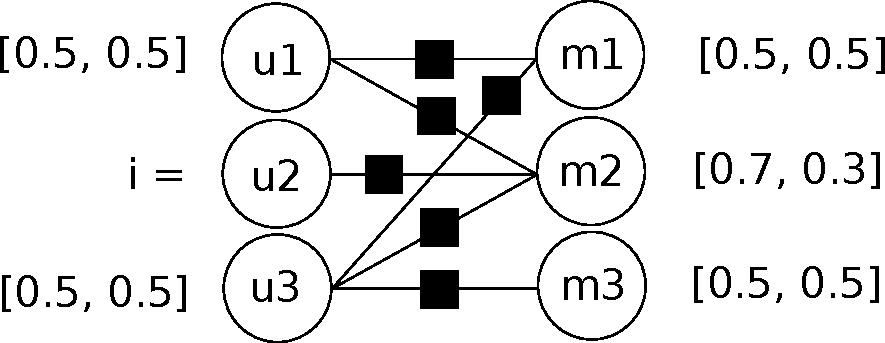
\includegraphics[scale=0.3]{graphics/top-n-graph.pdf}%
\caption{Factor Graph for predicting top-n movies for user $u_2$.
\label{top_n_graph}
}
\end{subfigure}\hfill%
\begin{subfigure}{.6\columnwidth}
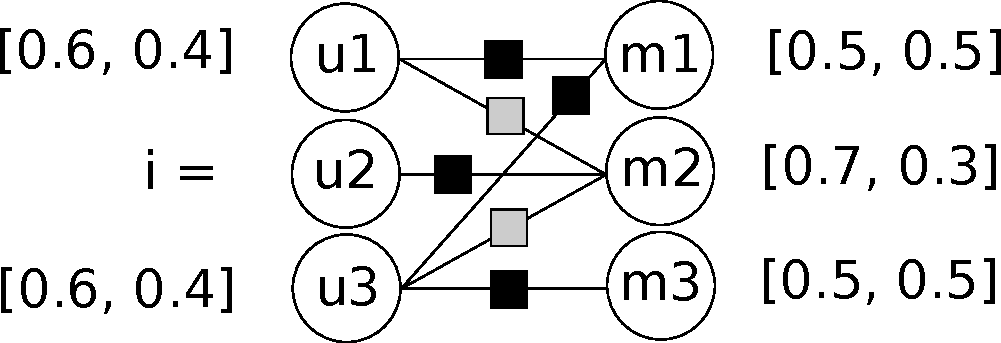
\includegraphics[scale=0.3]{graphics/top-n-important-messages.pdf}%
\caption{Belief is propagated from observed node $m_2$ to unobserved notes 
\label{top_n_graph_important_msg}
}
\end{subfigure}\hfill%
\begin{subfigure}{.6\columnwidth}
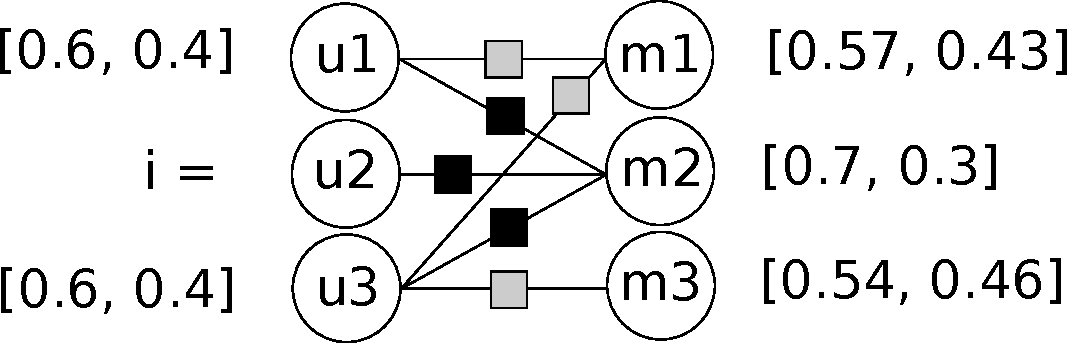
\includegraphics[scale=0.3]{graphics/top-n-final.pdf}%
\caption{A possible final state with $m_1$ being the top-1 recommendation for $u_2$. 
\label{top_n_graph_final_state}
}
\end{subfigure}
\caption{Top-N step by step}
\end{figure*}

\mypar{Cost Analysis}

Floating point operations are used as a cost measure, since the result of belief propagation is a list of probabilites which are represented as floating point numbers. Unfortunately, it is not possible to calculate the exact amount of floationg point operations for a given input size, as belief propagation is an iterative algorithm and the factor graph is heavily dependent on the input as it directly represents the user ratings. Therefore floating point operations are counted using performance counters. The following counters were used:

\begin{itemize}
	\item FP\_COMP\_OPS\_EXE.SSE\_SCALAR\_SINGLE and \\FP\_COMP\_OPS\_EXE.SSE\_SCALAR\_DOUBLE:\\count the number of SSE instructions on single floats and doubles.
	\item FP\_COMP\_OPS\_EXE.SSE\_PACKED\_SINGLE and \\FP\_COMP\_OPS\_EXE.SSE\_PACKED\_DOUBLE:\\count the number of packed SSE instructions on floats and doubles.
	\item SIMD\_FP\_256.PACKED\_SINGLE and \\SIMD\_FP\_256.PACKED\_DOUBLE:\\count the number of packed AVX instructions on floats and doubles.
	\item FP\_COMP\_OPS\_EXE.X87:\\counts the legacy X87 floating point instructions.
\end{itemize}

Since these counters do not allow to distinguish the operations (e.g separate additions from multiplications and divisions) all floating point operations are weighted the same. The performance counters were evaluated using VTune Amplifier XE 2015 (see section~\ref{sec:results}).

%\mypar{Discrete Fourier Transform}
%Precisely define the transform so I understand it even if I have never
%seen it before.
%
%\mypar{Fast Fourier Transforms}
%Explain the algorithm you use.
%
%\mypar{Cost Analysis}
%First define you cost measure (what you count) and then compute the
%cost. Ideally precisely, at least asymptotically. In the latter case you will need to instrument your code to count
%the operations so you can create a performance plot.
%
%Also state what is
%known about the complexity (asymptotic usually) 
%about your problem (including citations).